% I seguenti commenti speciali impostano:
% 1. 
% 2. PDFLaTeX come motore di composizione;
% 3. tesi.tex come documento principale;
% 4. il controllo ortografico italiano per l'editor.

% !TEX encoding = UTF-8
% !TEX TS-program = pdflatex
% !TEX root = tesi.tex
% !TEX spellcheck = it-IT
%!TEX program = xelatex
\documentclass[11pt,                    % corpo del font principale
    a4paper,                 % carta A4
    twoside,                 % impagina per fronte-retro
    openright,               % inizio capitoli a destra
    english,
    ctexart,
]{book}

%**************************************************************
% Importazione package
%************************************************************** 
%\usepackage{amsmath,amssymb,amsthm}    % matematica
\usepackage[UTF8]{ctex}
\usepackage[T1]{fontenc}                % codifica dei font:
% NOTA BENE! richiede una distribuzione *completa* di LaTeX

\usepackage[utf8]{inputenc}             % codifica di input; anche [latin1] va bene
% NOTA BENE! va accordata con le preferenze dell'editor

\usepackage[english]{babel}    % per scrivere in italiano e in inglese;
% l'ultima lingua (l'italiano) risulta predefinita

\usepackage{bookmark}                   % segnalibri

\usepackage{caption}                    % didascalie

\usepackage{chngpage,calc}              % centra il frontespizio

\usepackage{csquotes}                   % gestisce automaticamente i caratteri (")

\usepackage{emptypage}                  % pagine vuote senza testatina e piede di pagina

\usepackage{epigraph}            % per epigrafi

\usepackage{eurosym}                    % simbolo dell'euro

%\usepackage{indentfirst}               % rientra il primo paragrafo di ogni sezione

\usepackage{graphicx}                   % immagini

\usepackage{hyperref}                   % collegamenti ipertestuali

\usepackage[binding=5mm]{layaureo}      % margini ottimizzati per l'A4; rilegatura di 5 mm


\usepackage{microtype}                  % microtipografia

\usepackage{mparhack,fixltx2e,relsize}  % finezze tipografiche

\usepackage{nameref}                    % visualizza nome dei riferimenti                                      

\usepackage[font=small]{quoting}        % citazioni

%\usepackage{subfig}                     % sottofigure, sottotabelle

\usepackage[english]{varioref}          % riferimenti completi della pagina

\usepackage[dvipsnames]{xcolor}         % colori
\usepackage{formattazione}

\usepackage{booktabs}                   % tabelle                                       
\usepackage{tabularx}                   % tabelle di larghezza prefissata                                    
\usepackage{longtable}                  % tabelle su più pagine                                        
\usepackage{ltxtable}                   % tabelle su più pagine e adattabili in larghezza

\usepackage[toc, acronym]{glossaries}   % glossario
% per includerlo nel documento bisogna:
% 1. compilare una prima volta tesi.tex;
% 2. eseguire: makeindex -s tesi.ist -t tesi.glg -o tesi.gls tesi.glo
% 3. eseguire: makeindex -s tesi.ist -t tesi.alg -o tesi.acr tesi.acn
% 4. compilare due volte tesi.tex.

\usepackage[backend=biber,style=numeric-comp,hyperref,backref]{biblatex}
% eccellente pacchetto per la bibliografia;
% produce uno stile di citazione autore-anno;
% lo stile "numeric-comp" produce riferimenti numerici
% per includerlo nel documento bisogna:
% 1. compilare una prima volta tesi.tex;
% 2. eseguire: biber tesi
% 3. compilare ancora tesi.tex.

%**************************************************************
% file contenente le impostazioni della tesi
%**************************************************************

%**************************************************************
% Frontespizio
%**************************************************************

% Autore
\newcommand{\myName}{Xiaowei Wen}
\newcommand{\myTitle}{Transformer applied to Visual Odometry}

% Tipo di tesi                   
\newcommand{\myDegree}{Master degree thesis}

% Università             
\newcommand{\myUni}{Alma Mater Studiorum - University of Bologna}

% Facoltà       
\newcommand{\myFaculty}{Artificial Intelligence}

% Dipartimento
\newcommand{\myDepartment}{Computer Science and Engineering - DISI}

% Titolo del relatore
\newcommand{\profTitle}{Prof.}

% Relatore
\newcommand{\myProf}{ Luigi Di Stefano}

% Luogo
\newcommand{\myLocation}{Bologna}

% Anno accademico
\newcommand{\myAA}{2021-2022}

% Data discussione
\newcommand{\myTime}{06 October 2022}


\addto\captionsenglish{\renewcommand{\lstlistingname}{Code}}

%**************************************************************
% Impostazioni di impaginazione
% see: http://wwwcdf.pd.infn.it/AppuntiLinux/a2547.htm
%**************************************************************

\setlength{\parindent}{14pt}   % larghezza rientro della prima riga
\setlength{\parskip}{0pt}   % distanza tra i paragrafi


%**************************************************************
% Impostazioni di biblatex
%**************************************************************
\bibliography{bibliografia} % database di biblatex 

\defbibheading{bibliography} {
    \cleardoublepage
    \phantomsection 
    \addcontentsline{toc}{chapter}{\bibname}
    \chapter*{\bibname\markboth{\bibname}{\bibname}}
}

\setlength\bibitemsep{1.5\itemsep} % spazio tra entry

\DeclareBibliographyCategory{opere}
\DeclareBibliographyCategory{web}

\addtocategory{opere}{womak:lean-thinking}
\addtocategory{web}{site:agile-manifesto}

\defbibheading{opere}{\section*{Bibliography}}
\defbibheading{web}{\section*{Websites}}


%**************************************************************
% Impostazioni di caption
%**************************************************************
\captionsetup{
    tableposition=top,
    figureposition=bottom,
    font=small,
    format=hang,
    labelfont=bf
}

%**************************************************************
% Impostazioni di glossaries
%**************************************************************
\input{Glossario} % database di termini
\makeglossaries


%**************************************************************
% Impostazioni di graphicx
%**************************************************************
\graphicspath{{images/}} % cartella dove sono riposte le immagini


%**************************************************************
% Impostazioni di hyperref
%**************************************************************
\hypersetup{
    %hyperfootnotes=false,
    %pdfpagelabels,
    %draft,	% = elimina tutti i link (utile per stampe in bianco e nero)
    colorlinks=true,
    linktocpage=true,
    pdfstartpage=1,
    pdfstartview=FitV,
    % decommenta la riga seguente per avere link in nero (per esempio per la stampa in bianco e nero)
    %colorlinks=false, linktocpage=false, pdfborder={0 0 0}, pdfstartpage=1, pdfstartview=FitV,
    breaklinks=true,
    pdfpagemode=UseNone,
    pageanchor=true,
    pdfpagemode=UseOutlines,
    plainpages=false,
    bookmarksnumbered,
    bookmarksopen=true,
    bookmarksopenlevel=1,
    hypertexnames=true,
    pdfhighlight=/O,
    %nesting=true,
    %frenchlinks,
    urlcolor=webbrown,
    linkcolor=RoyalBlue,
    citecolor=webgreen,
    %pagecolor=RoyalBlue,
    %urlcolor=Black, linkcolor=Black, citecolor=Black, %pagecolor=Black,
    pdftitle={\myTitle},
    pdfauthor={\textcopyright\ \myName, \myUni, \myFaculty},
    pdfsubject={},
    pdfkeywords={},
    pdfcreator={pdfLaTeX},
    pdfproducer={LaTeX}
}

%**************************************************************
% Impostazioni di itemize
%**************************************************************
%\renewcommand{\labelitemi}{$\ast$}

%\renewcommand{\labelitemi}{$\bullet$}
%\renewcommand{\labelitemii}{$\cdot$}
%\renewcommand{\labelitemiii}{$\diamond$}
%\renewcommand{\labelitemiv}{$\ast$}


%**************************************************************
% Impostazioni di listings
%**************************************************************
\lstset{
    language=[LaTeX]Tex,%C++,
    keywordstyle=\color{RoyalBlue}, %\bfseries,
    basicstyle=\small\ttfamily,
    %identifierstyle=\color{NavyBlue},
    commentstyle=\color{Green}\ttfamily,
    stringstyle=\rmfamily,
    numbers=none, %left,%
    numberstyle=\scriptsize, %\tiny
    stepnumber=5,
    numbersep=8pt,
    showstringspaces=false,
    breaklines=true,
    frameround=ftff,
    frame=single
} 


%**************************************************************
% Impostazioni di xcolor
%**************************************************************
\definecolor{webgreen}{rgb}{0,.5,0}
\definecolor{webbrown}{rgb}{.6,0,0}
\usepackage{chngcntr}
\counterwithout{footnote}{chapter}

%**************************************************************
% Altro
%**************************************************************

\newcommand{\omissis}{[\dots\negthinspace]} % produce [...]

% eccezioni all'algoritmo di sillabazione
\hyphenation
{
    ma-cro-istru-zio-ne
    gi-ral-din
}

\newcommand{\sectionname}{Section}
\addto\captions{\renewcommand{\figurename}{Figure}
                       \renewcommand{\tablename}{Table}}

\newcommand{\glsfirstoccur}{\ap{{[g]}}}

\newcommand{\intro}[1]{\emph{\textsf{#1}}}

%**************************************************************
% Environment per ``namespace description''
%**************************************************************

\newenvironment{namespacedesc}{
    \vspace{10pt}
    \par \noindent                              % start new paragraph
    \begin{description} 
}{
    \end{description}
    \medskip
}

\newcommand{\classdesc}[2]{\item[\textbf{#1:}] #2}
\renewcommand{\labelitemi}{$\bullet$}
\renewcommand{\labelitemii}{$\circ$}
\renewcommand{\labelitemiii}{-}
\renewcommand{\labelitemiv}{$\cdot$}
                     % file con le impostazioni personali
\raggedbottom
\begin{document}
%**************************************************************
% Materiale iniziale
%**************************************************************
    \frontmatter
    % !TEX encoding = UTF-8
% !TEX TS-program = pdflatex
% !TEX root = ../tesi.tex

%**************************************************************
% Frontespizio 
%**************************************************************
\begin{titlepage}

\begin{center}

\begin{LARGE}
\textbf{\myUni}\\
\end{LARGE}

\vspace{10pt}

\begin{Large}
\textsc{\myDepartment}\\
\end{Large}

\vspace{10pt}

\begin{large}
\textsc{\myFaculty}\\
\end{large}

\vspace{250pt}
%\begin{figure}[htbp]
%\begin{center}
%%\includegraphics[height=6cm]{logo}
%\end{center}
%\end{figure}
%\vspace{30pt}

\begin{LARGE}
\begin{center}
\textbf{\myTitle}\\
\end{center}
\end{LARGE}

\vspace{10pt} 

\begin{large}
\textsl{\myDegree}\\
\end{large}

\vspace{40pt}

\begin{large}
\begin{flushleft}
\textit{Relatore}\\ 
\vspace{5pt} 
\profTitle \myProf
\end{flushleft}

\vspace{0pt} 

\begin{flushright}
\textit{Laureando}\\ 
\vspace{5pt} 
\myName
\end{flushright}
\end{large}

\vspace{20pt}

\line(1, 0){338} \\
\begin{normalsize}
\textsc{Anno Accademico \myAA - Second session}
\end{normalsize}

\end{center}
    \end{titlepage}
    % !TEX encoding = UTF-8
% !TEX TS-program = pdflatex
% !TEX root = ../tesi.tex

%**************************************************************
% Colophon
%**************************************************************
\clearpage
\phantomsection
\thispagestyle{empty}

\hfill

\vfill

\noindent\myName: \textit{\myTitle,}
\myDegree,
\textcopyright\ \myTime.
    % !TEX encoding = UTF-8
% !TEX TS-program = pdflatex
% !TEX root = ../tesi.tex

%**************************************************************
% Dedica
%**************************************************************
\cleardoublepage
\phantomsection
\thispagestyle{empty}
\pdfbookmark{Dedica}{Dedica}

\vspace*{3cm}

\begin{center}
%    "Così come in algebra due affermazioni false ne danno una vera, così spero che il prodotto dei miei insuccessi si concluda con un successo." \medskip
%    --V. Van Gogh
\end{center}

\medskip

\begin{center}
Dedicated to my parents.
\end{center}

    % !TEX encoding = UTF-8
% !TEX TS-program = pdflatex
% !TEX root = ../tesi.tex

%**************************************************************
% Sommario
%**************************************************************
\cleardoublepage
\phantomsection
\pdfbookmark{Summary}{Summary}
\begingroup
\let\clearpage\relax
\let\cleardoublepage\relax
\let\cleardoublepage\relax

\chapter*{Summary}

%\vfill
%
%\selectlanguage{english}
%\pdfbookmark{Abstract}{Abstract}
%\chapter*{Abstract}
%
%\selectlanguage{italian}
This dissertation describes a deepening study about Visual Odometry problem tackled with transformer architectures.
The initial objectives were: create a synthetic dataset using BlenderProc2 framework, try different versions of transformer architectures which includes:
ResNet feature-extractor with encoder, ResNet feature-extractor with encoder-decoder, ResNet-feature extractor with encoder-decoder and pose Auto-encoder.


\endgroup			

\vfill


    % !TEX encoding = UTF-8
% !TEX TS-program = pdflatex
% !TEX root = ../tesi.tex

%**************************************************************
% Ringraziamenti
%**************************************************************
\cleardoublepage
\phantomsection
\pdfbookmark{Thanks}{Thanks}
\begin{flushright}{
	\slshape
	``Dio benedica quelle persone che quando incroci il loro sguardo per sbaglio, sorridono.''} \\
	\medskip
\end{flushright}


\bigskip

\begingroup
\let\clearpage\relax
\let\cleardoublepage\relax
\let\cleardoublepage\relax

\chapter*{Thanks}

\noindent \textit{Innanzitutto, vorrei esprimere la mia gratitudine al Prof. Sperduti, relatore della mia tesi, e Alessandro Proscia, il tutor aziendale, per l'aiuto e il sostegno fornitomi durante la stesura del lavoro.}\\

\noindent \textit{Desidero ringraziare con affetto i miei genitori per il sostegno, il grande aiuto e per essermi stati vicini in ogni momento durante gli anni di studio.}\\

\noindent \textit{Ho desiderio di ringraziare poi Veronica, Alberto, Marco, Lorenzo, Linpeng, Tommaso, Alessandro e Giulio per tutti i bellissimi anni passati insieme, le avventure vissute e di essersi sorbiti mille delle mie lamentele.}\\

\noindent \textit{Infine, vorrei esprimere la mia gratitudine alla famiglia Geminian e Bernardi per tutti gli aiuti ricevuti durante questi anni.}\\
\bigskip

\noindent\textit{\myLocation, \myTime}
\hfill \myName

\endgroup


    % !TEX encoding = UTF-8
% !TEX TS-program = pdflatex
% !TEX root = ../tesi.tex

%**************************************************************
% Indici
%**************************************************************
\cleardoublepage
\pdfbookmark{\contentsname}{tableofcontents}
\setcounter{tocdepth}{2}
\tableofcontents
%\markboth{\contentsname}{\contentsname} 
\clearpage

\begingroup 
    \let\clearpage\relax
    \let\cleardoublepage\relax
    \let\cleardoublepage\relax
    %*******************************************************
    % Elenco delle figure
    %*******************************************************    
    \phantomsection
    \pdfbookmark{\listfigurename}{lof}
    \listoffigures

    \vspace*{8ex}

    %*******************************************************
    % Elenco delle tabelle
    %*******************************************************
    \phantomsection
    \pdfbookmark{\listtablename}{lot}
    \listoftables
    \vspace*{8ex}
\endgroup

\cleardoublepage

    \cleardoublepage

%**************************************************************
% Materiale principale
%**************************************************************
    \mainmatter
    % !TEX encoding = UTF-8
% !TEX TS-program = pdflatex
% !TEX root = ../tesi.tex

%**************************************************************
\chapter{Introduzione}\label{ch:introduzione}
%**************************************************************

\intro{In questa sezione viene svolta una breve introduzione alle idee dello stage e una breve presentazione dell'azienda Imola Informatica S.p.A.}
%\noindent Esempio di utilizzo di un termine nel glossario \\
%\gls{api}. \\
%
%\noindent Esempio di citazione in linea \\
%\cite{site:agile-manifesto}. \\
%
%\noindent Esempio di citazione nel pie' di pagina \\
%citazione\footcite{womak:lean-thinking} \\

%\input{capitoli/1_1_idea}
%\input{capitoli/1_2_introduzione_al_progetto}
%\input{capitoli/1_3_azienda}
%\input{capitoli/1_4_risultati.tex}
%\input{capitoli/1_5_organizzazione_del_testo.tex}
             % Introduzione         % Kick-Off
    % !TEX encoding = UTF-8
% !TEX TS-program = pdflatex
% !TEX root = ../tesi.tex

%**************************************************************

\chapter{Theoretical foundations}
\label{ch:theoretical-foundations}
%**************************************************************

\intro{In this chapter will be presented the main theoretical knowledge useful to understand the content from successive chapters.}\\

\section{Deep Learning}\label{sec:deep-learning}


A deep neural network is composed mainly by the neural network, the optimizer, the loss function, meanwhile, there are also other components, like learning rate lr scheduler, which can change the value of the learning rate during the training based on the value of the loss function.

The Neural network can be composed by different layers, e.g., the dense layer, the convolutional layer, the pooling layer, the layers between the first and the last are called hidden layers.
After each layer, there is the activation function, for example can be: relu, gelu, selu, leakyRelu,  % esempi con le activation funcitons.
\subsection{Convolutional Neural Network}\label{subsec:conv-neural-network}

\subsection{Transformer}\label{subsec:transformer}

\section{Visual Odometry}\label{sec:visual-odometry}

Visual Odometry is an important task in robotics' computer vision field, because it allows the robot to understand where it is and how it is oriented.
%\input{./chapters/4_3_progettazione.tex}
%\input{./chapters/4_4_design_pattern_utilizzati.tex}
%\input{./chapters/4_5_codifica.tex}             % Product Prototype
    % !TEX encoding = UTF-8
% !TEX TS-program = pdflatex
% !TEX root = ../tesi.tex

%**************************************************************
\section{Kitti}
\label{sec:kitti}
%**************************************************************

The odometry benchmark consists of 22 stereo sequences, saved in loss less png format: 11 sequences are provided with ground truth trajectories for training and 11 sequences (11-21) without ground truth trajectories for evaluation.

This odometry benchmark is a subset of KITTI Vision Benchmark suite. % todo aggiungere reference al paper http://www.cvlibs.net/publications/Geiger2012CVPR.pdf

\subsection{Scene}\label{subsec:kitti-scene}
The images represents a various of scenes from mid-sized city, rural areas and on highways.
\begin{figure}[H]
    \centering
    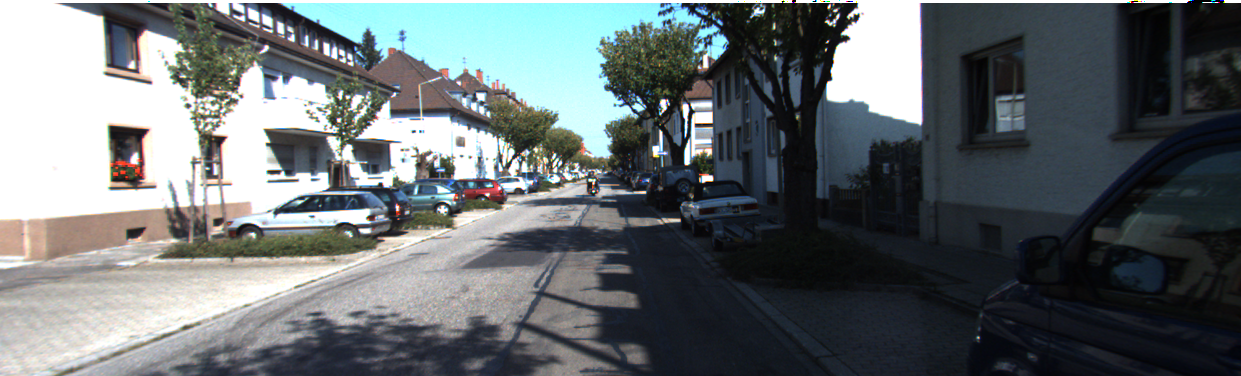
\includegraphics[width=\textwidth]{images/3_1_example_kitti_scene}
    \caption{KITTI - example of scene}\label{fig:example-of-kitti-scene}
\end{figure}

\subsection{Image generation}\label{subsec:kitti-image-generation}
Each sequence of the KITTI dataset is composed of by four sequences of images: left-coloured, right-coloured, left-grey and right-grey.
Each one is captured by a camera mounted on the top of vehicle.
They calibrated the four video cameras intrinsically and extrinsically and rectified the input image.
Then they computed the 3D rigid motion parameters which relate the coordinate system of the laser scanner.

Meanwhile, the ground-truth is directly given by the output of the GPS/IMU localization unit projected into the coordinate system of the left camera after rectification.

\subsection{Dataset statistics}\label{subsec:kitti-dataset-statistics}
The dataset consists of 22 stereo sequences, with a total length of 39.2 km, which was the longest in the time of the publication of the paper.
In the dataset, there are no specifically indicate which sequence is used for training, validation or testing, but in this work, the dataset is split as this:
\begin{table}[H]
    \centering
    \begin{tabular}{|c|c|c|}
        \hline
        \textbf{Sets}           & \textbf{N. of Sequence} & \textbf{N. Image} \\ \hline
        \textbf{Training set}   & 8                       & 20.098            \\ \hline
        \textbf{Validation set} & 2                       & 1.902             \\ \hline
        \textbf{Test set}       & 1                       & 1.201             \\ \hline
        \textit{\textbf{Total}} & 11                      & 23.201            \\ \hline
    \end{tabular}\caption{KITTI - dataset statistics}\label{tab:kitti-dataset-statistics}
\end{table}

The images dimensions about 1240x370 are slightly different, generally varying for few pixels.
\subsection{Usage}\label{subsec:kitti-usage}

This dataset is the one mainly used, as it is the one of the most famous and most used in the literature.

The sequence \textbf{3} and \textbf{7} are used for evaluation and testing, because they are the easier ones.
\begin{figure}[H]
    \centering
    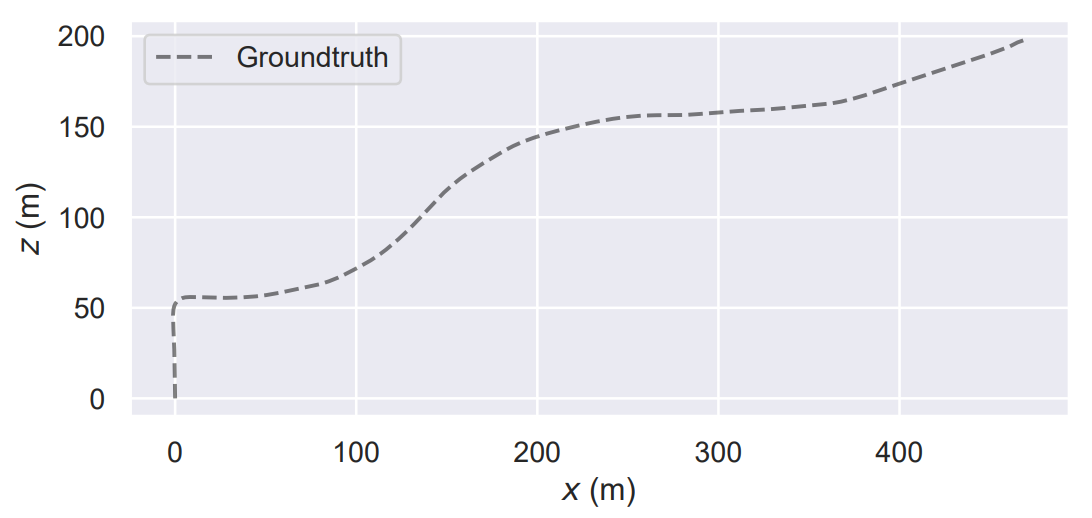
\includegraphics[width=0.5\textwidth]{images/3_1_kitti_seq_3}
    \caption{KITTI - sequence 3}\label{fig:kitti-seq-3}
\end{figure}
\begin{figure}[H]
    \centering
    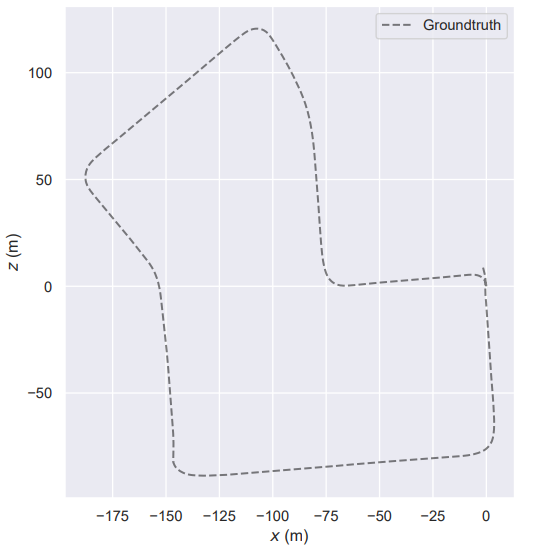
\includegraphics[width=0.5\textwidth]{images/3_1_kitti_seq_7}
    \caption{KITTI - sequence 7}\label{fig:kitti-seq-7}
\end{figure}

Initially, to test the model's capacity, the model was trained and evaluated on the same sequence, to see if it's able to reproduce the ground truth.
Then, the model was fed with more complex sequences.             % Concept Preview
    % !TEX encoding = UTF-8
% !TEX TS-program = pdflatex
% !TEX root = ../tesi.tex

%**************************************************************
\chapter{Datasets}
\label{ch:datasets}
\intro{In this chapter will be presented the datasets created and used for the visual odometry.}

%%**************************************************************
%
% !TEX encoding = UTF-8
% !TEX TS-program = pdflatex
% !TEX root = ../tesi.tex

%**************************************************************
\section{Kitti}
\label{sec:kitti}
%**************************************************************

The odometry benchmark consists of 22 stereo sequences, saved in loss less png format: 11 sequences are provided with ground truth trajectories for training and 11 sequences (11-21) without ground truth trajectories for evaluation.

This odometry benchmark is a subset of KITTI Vision Benchmark suite. % todo aggiungere reference al paper http://www.cvlibs.net/publications/Geiger2012CVPR.pdf

\subsection{Scene}\label{subsec:kitti-scene}
The images represents a various of scenes from mid-sized city, rural areas and on highways.
\begin{figure}[H]
    \centering
    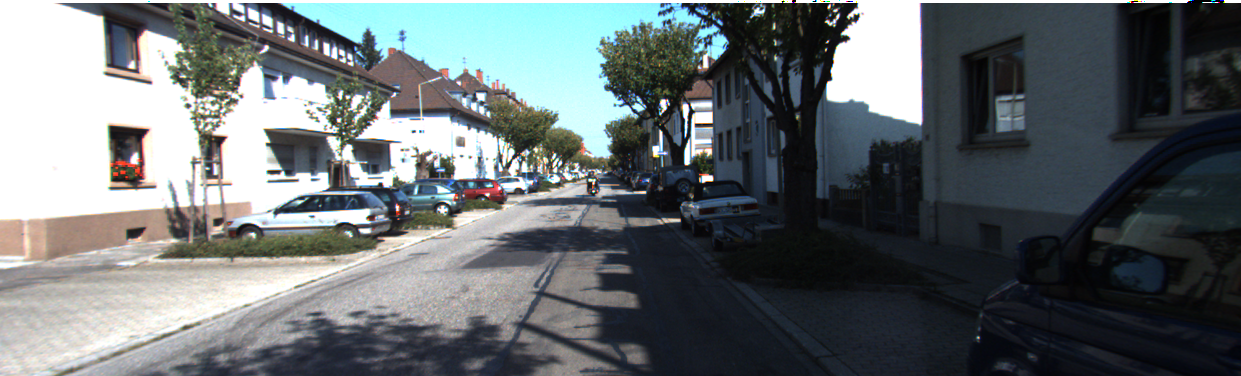
\includegraphics[width=\textwidth]{images/3_1_example_kitti_scene}
    \caption{KITTI - example of scene}\label{fig:example-of-kitti-scene}
\end{figure}

\subsection{Image generation}\label{subsec:kitti-image-generation}
Each sequence of the KITTI dataset is composed of by four sequences of images: left-coloured, right-coloured, left-grey and right-grey.
Each one is captured by a camera mounted on the top of vehicle.
They calibrated the four video cameras intrinsically and extrinsically and rectified the input image.
Then they computed the 3D rigid motion parameters which relate the coordinate system of the laser scanner.

Meanwhile, the ground-truth is directly given by the output of the GPS/IMU localization unit projected into the coordinate system of the left camera after rectification.

\subsection{Dataset statistics}\label{subsec:kitti-dataset-statistics}
The dataset consists of 22 stereo sequences, with a total length of 39.2 km, which was the longest in the time of the publication of the paper.
In the dataset, there are no specifically indicate which sequence is used for training, validation or testing, but in this work, the dataset is split as this:
\begin{table}[H]
    \centering
    \begin{tabular}{|c|c|c|}
        \hline
        \textbf{Sets}           & \textbf{N. of Sequence} & \textbf{N. Image} \\ \hline
        \textbf{Training set}   & 8                       & 20.098            \\ \hline
        \textbf{Validation set} & 2                       & 1.902             \\ \hline
        \textbf{Test set}       & 1                       & 1.201             \\ \hline
        \textit{\textbf{Total}} & 11                      & 23.201            \\ \hline
    \end{tabular}\caption{KITTI - dataset statistics}\label{tab:kitti-dataset-statistics}
\end{table}

The images dimensions about 1240x370 are slightly different, generally varying for few pixels.
\subsection{Usage}\label{subsec:kitti-usage}

This dataset is the one mainly used, as it is the one of the most famous and most used in the literature.

The sequence \textbf{3} and \textbf{7} are used for evaluation and testing, because they are the easier ones.
\begin{figure}[H]
    \centering
    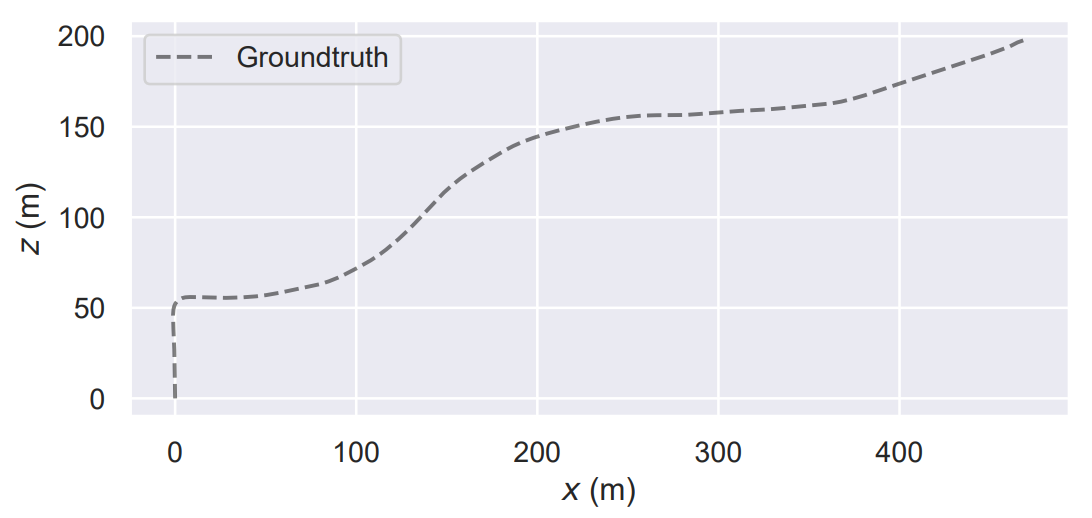
\includegraphics[width=0.5\textwidth]{images/3_1_kitti_seq_3}
    \caption{KITTI - sequence 3}\label{fig:kitti-seq-3}
\end{figure}
\begin{figure}[H]
    \centering
    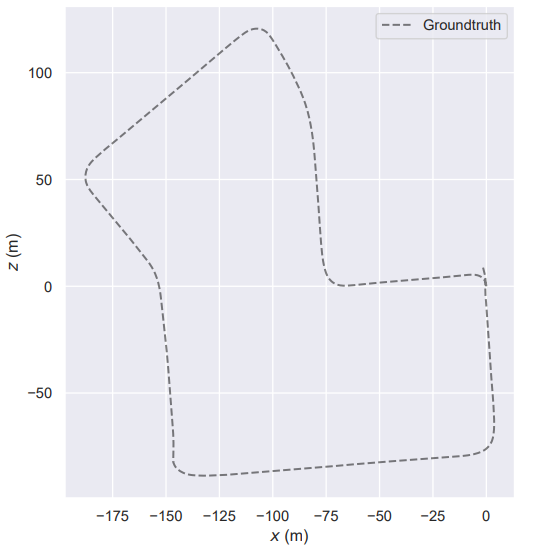
\includegraphics[width=0.5\textwidth]{images/3_1_kitti_seq_7}
    \caption{KITTI - sequence 7}\label{fig:kitti-seq-7}
\end{figure}

Initially, to test the model's capacity, the model was trained and evaluated on the same sequence, to see if it's able to reproduce the ground truth.
Then, the model was fed with more complex sequences.
%
%%**************************************************************
%
% !TEX encoding = UTF-8
% !TEX TS-program = pdflatex
% !TEX root = ./tesi.tex

%**************************************************************
\section{Synthetic}\label{sec:synthetic}
%**************************************************************

As in there are few real-life datasets for visual odometry, we decided to create a synthetic dataset by using BlenderProc2 framework,
which is a procedural photo-realistic rendering framework, and it allows to:
\begin{itemize}
    \item \textbf{Loading}: *\textit{.obj}, *\textit{.ply}, *\textit{.blend}, \textit{BOP}, \textit{ShapeNet} etc.
    \item \textbf{Objects}: set or sample objects poses, apply physics and collision checking.
    \item \textbf{Materials}: set or sample physically-based materials and textures.
    \item \textbf{Lighting}: set or sample lights, automatic lighting of 3D-front scenes.
    \item \textbf{Cameras}: set, sample or load camera poses from file.
    \item \textbf{Rendering}: RGB, stereo, depth, normal and segmentation images/sequences.
    \item \textbf{Writing}: *.hdf5 containers, \textit{COCO} and \textit{BOP} annotations.
\end{itemize}

\subsection{Scene}\label{subsec:scene}
To create the synthetic dataset, the first thing is to create a scene with customized objects, material and textures.
\begin{figure}[H]
    \centering
    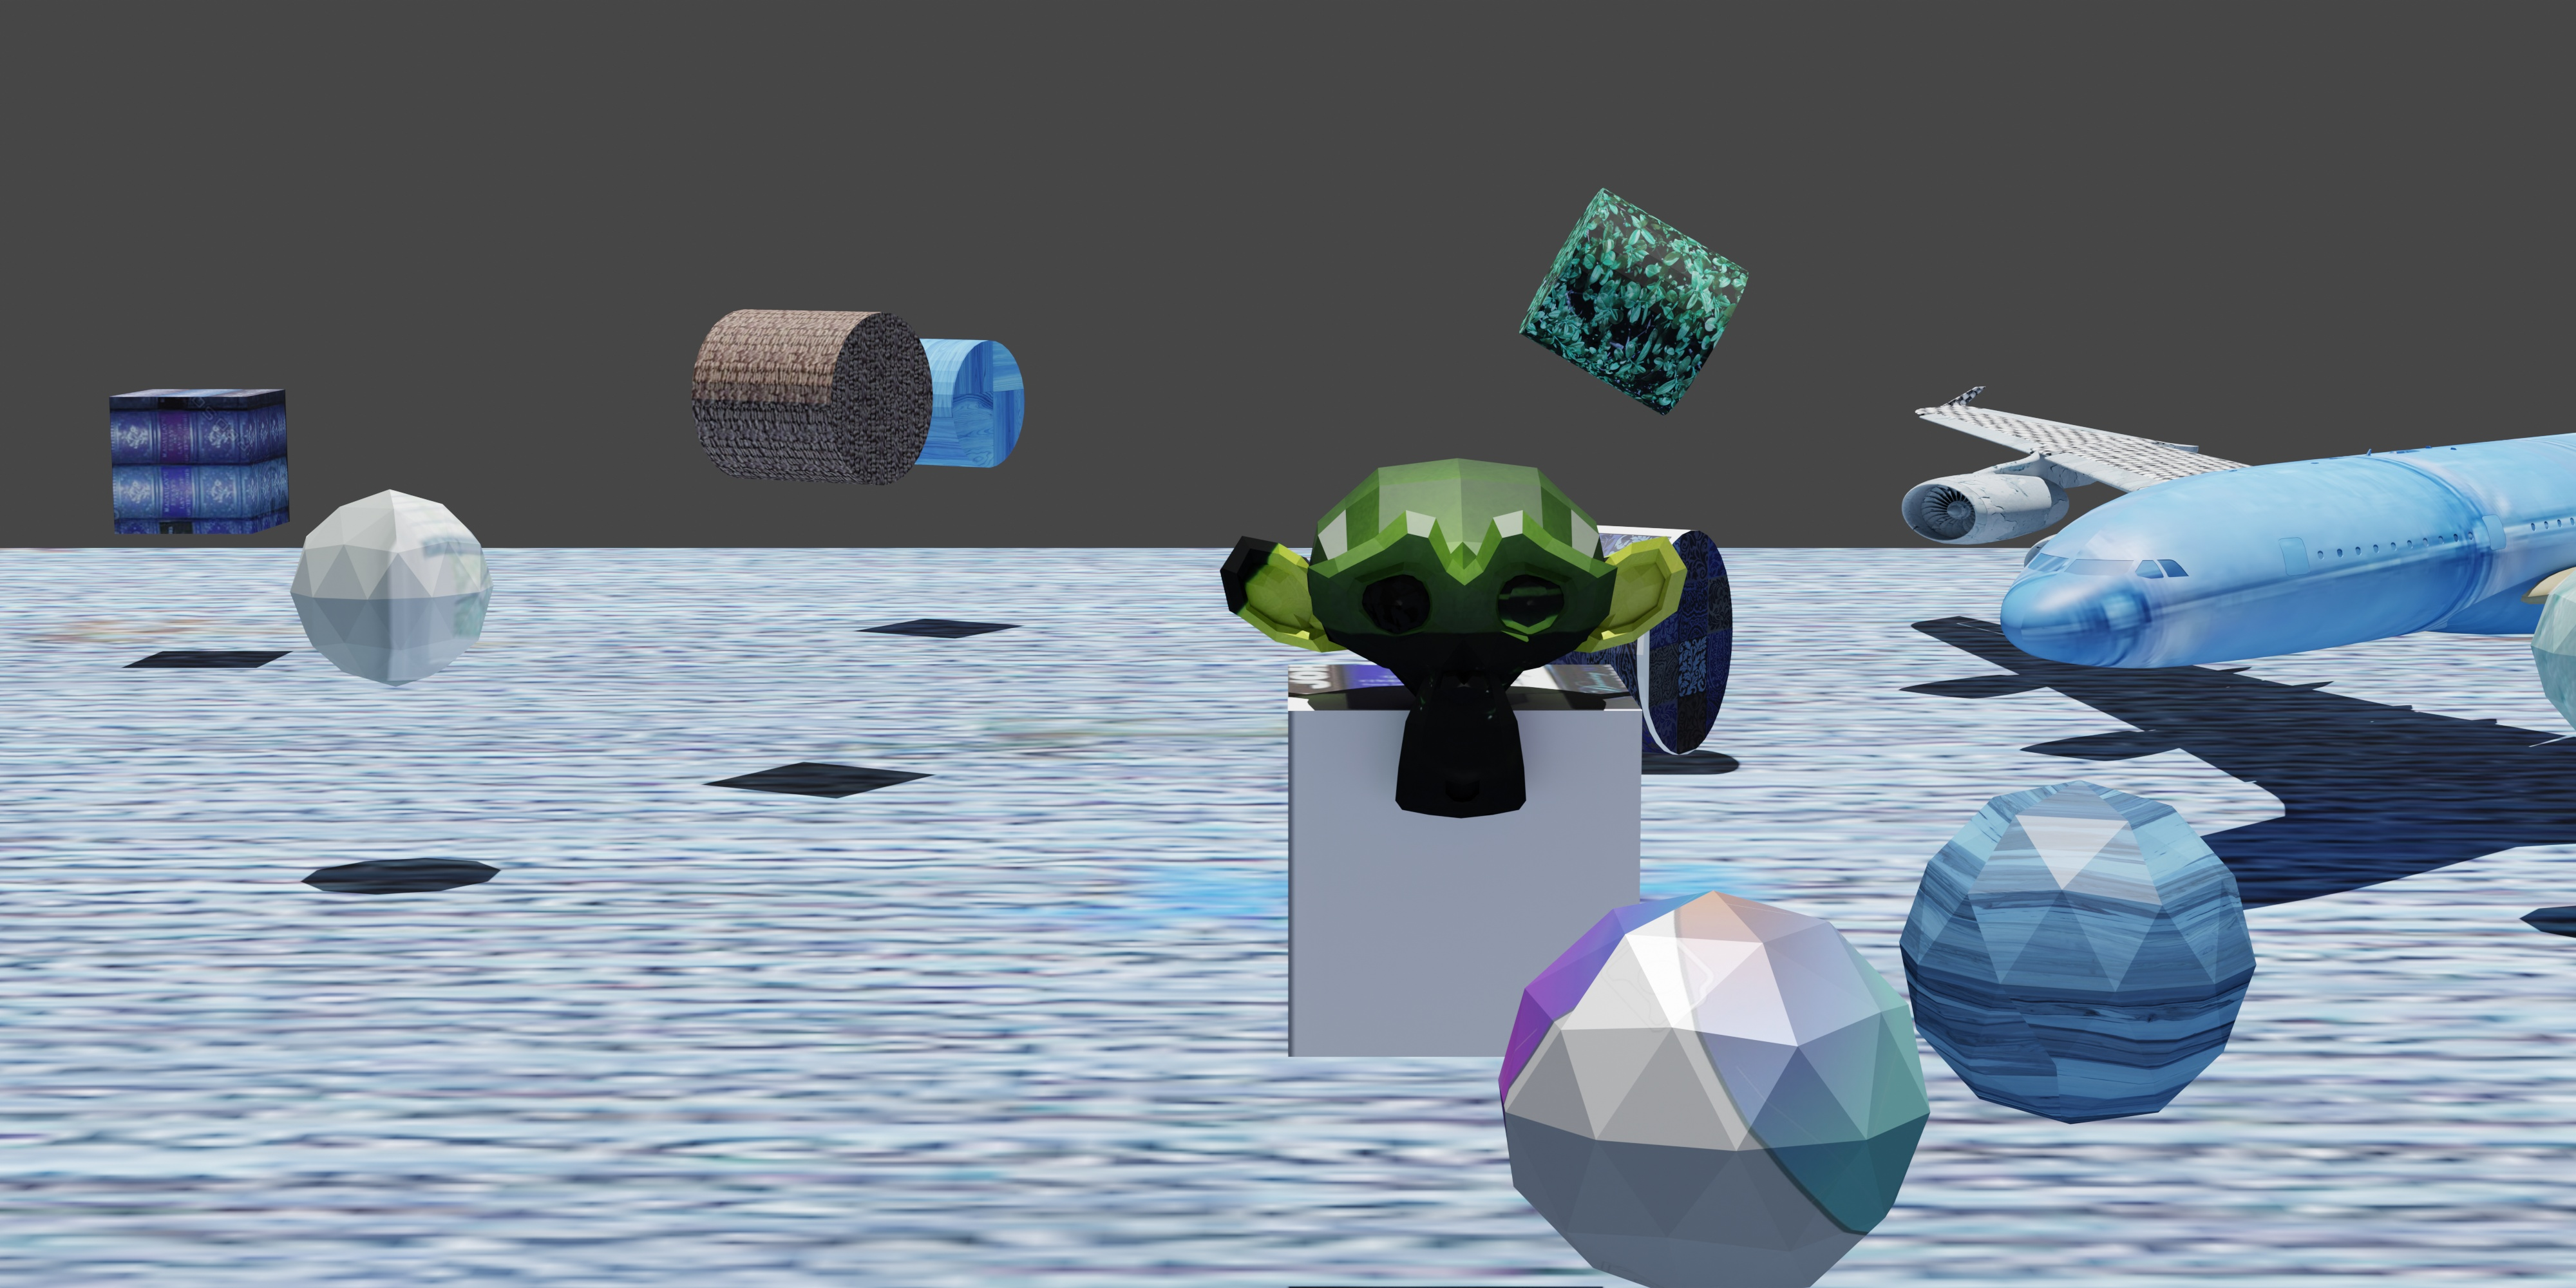
\includegraphics[width=\textwidth]{images/3_example_of_scene}
    \caption{Example of scene}\label{fig:example-of-scene}
\end{figure}
The scene is composed by a set of objects, more precisely:
\begin{itemize}
    \item \textbf{a monkey}: which is at the centre of the scene over a cube.
    \item \textbf{a plane}: which is at left corner of the scene.
    \item \textbf{a set of cubes and spheres}: which are placed randomly in the scene.
\end{itemize}

When rendering the scene, the textures are loaded \textit{randomly}, in the way that in different sequences the textures are different.
\subsection{Image generation}\label{subsec:image-generation}
To generate the sequences, we need to choose the camera position in the scene to do so, we choose randomly a position sampler from the following set for each new pose:

\begin{itemize}
    \item \textbf{disk}: samples a point on a circle or on a 2-ball or on an arc/sector with an inner angle less or equal to 180 degrees.
    \item \textbf{sphere}: samples a point from the surface or from the interior of a solid sphere.
    \item \textbf{part-sphere}: samples a point from the surface or from the interior of a solid sphere which is split in two parts.
    \item \textbf{shell}: samples a point from the volume between two spheres (with radius of the spheres given as parameters).
\end{itemize}
once we have the next position of the camera, we compute the rotation matrix to be applied to the camera in the way that the camera is always looking at the POI (Point Of Interest) which corresponds to the centre of the scene.
\begin{lstlisting}[label={lst:compute-camera-rotation}, caption={Computes the rotatition matrix for the camera.}, captionpos=b]
rotation = bproc.camera.rotation_from_forward_vec(poi - new_position)
\end{lstlisting}
Then, we apply the rotation matrix to the camera and we generate the image, and by setting a certain number of frames between two poses, the framework renders a sequence of images with relative intermediate poses.


But sometime, it happens that the new camera pose is too close to an object of the scene, so we set two conditions that need to be satisfied, otherwise the sampled camera pose is skipped.
The first condition checks if there are obstacles in front of the camera which are too far or too close based on the given \textit{proximity\_checks}, while the second evaluates the interestingness or coverage of the scene.
\begin{lstlisting}[label={lst:lstlisting}, caption={Checks whether the camera pose satisfies the conditions.}, captionpos=b]
def check_pose(c2w_m, special_obj, bvh_tree):
    if not bproc.camera.perform_obstacle_in_view_check(c2w_m, {"min": 5.0}, bvh_tree):
        return False
    if bproc.camera.scene_coverage_score(c2w_m, special_objects=special_obj) < 0.7:
        return False
    return True
\end{lstlisting}


But when the new position is to far away from the old position, the rotation of the camera assumes a wrong value during the transition, because it rotates counter-clockwise instead of clockwise, or vice-versa.
For example:
If we sample the camera position from a disk at 0, 90, 180, 270 degrees, the rotations should be as in the figure 3.1:
\begin{figure}[H]
    \centering
    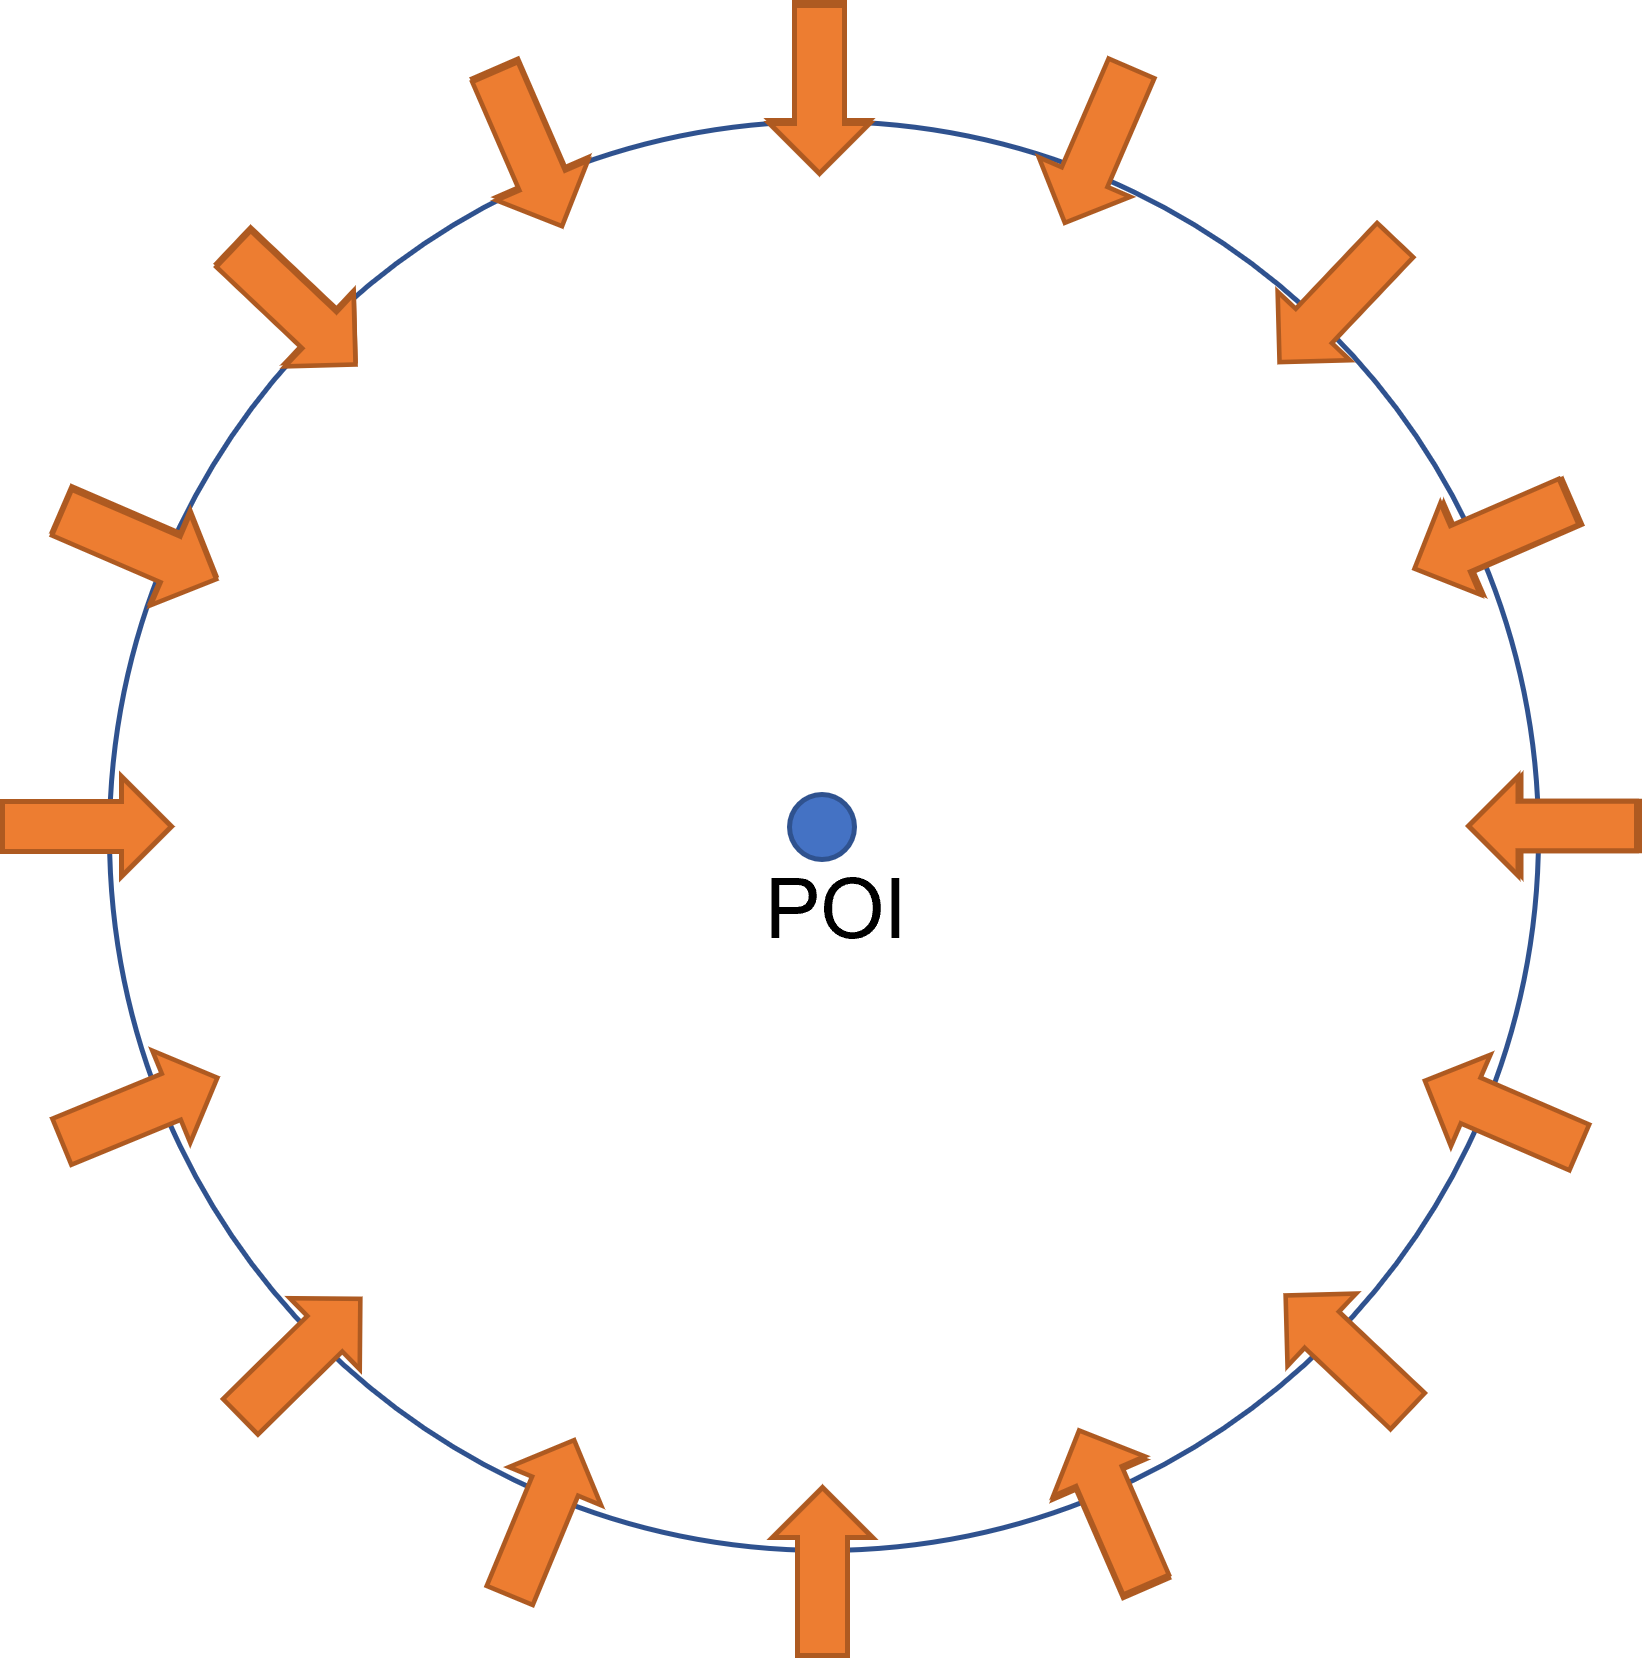
\includegraphics[width=0.5\textwidth]{images/3_correct_transitions}
    \caption{Correct transition on the disk}\label{fig:correct-transition}
\end{figure}

But, the transition from 180 to 270 degrees we obtain is a wrong rotation which is like in figure 3.2:
\begin{figure}[H]
    \centering
    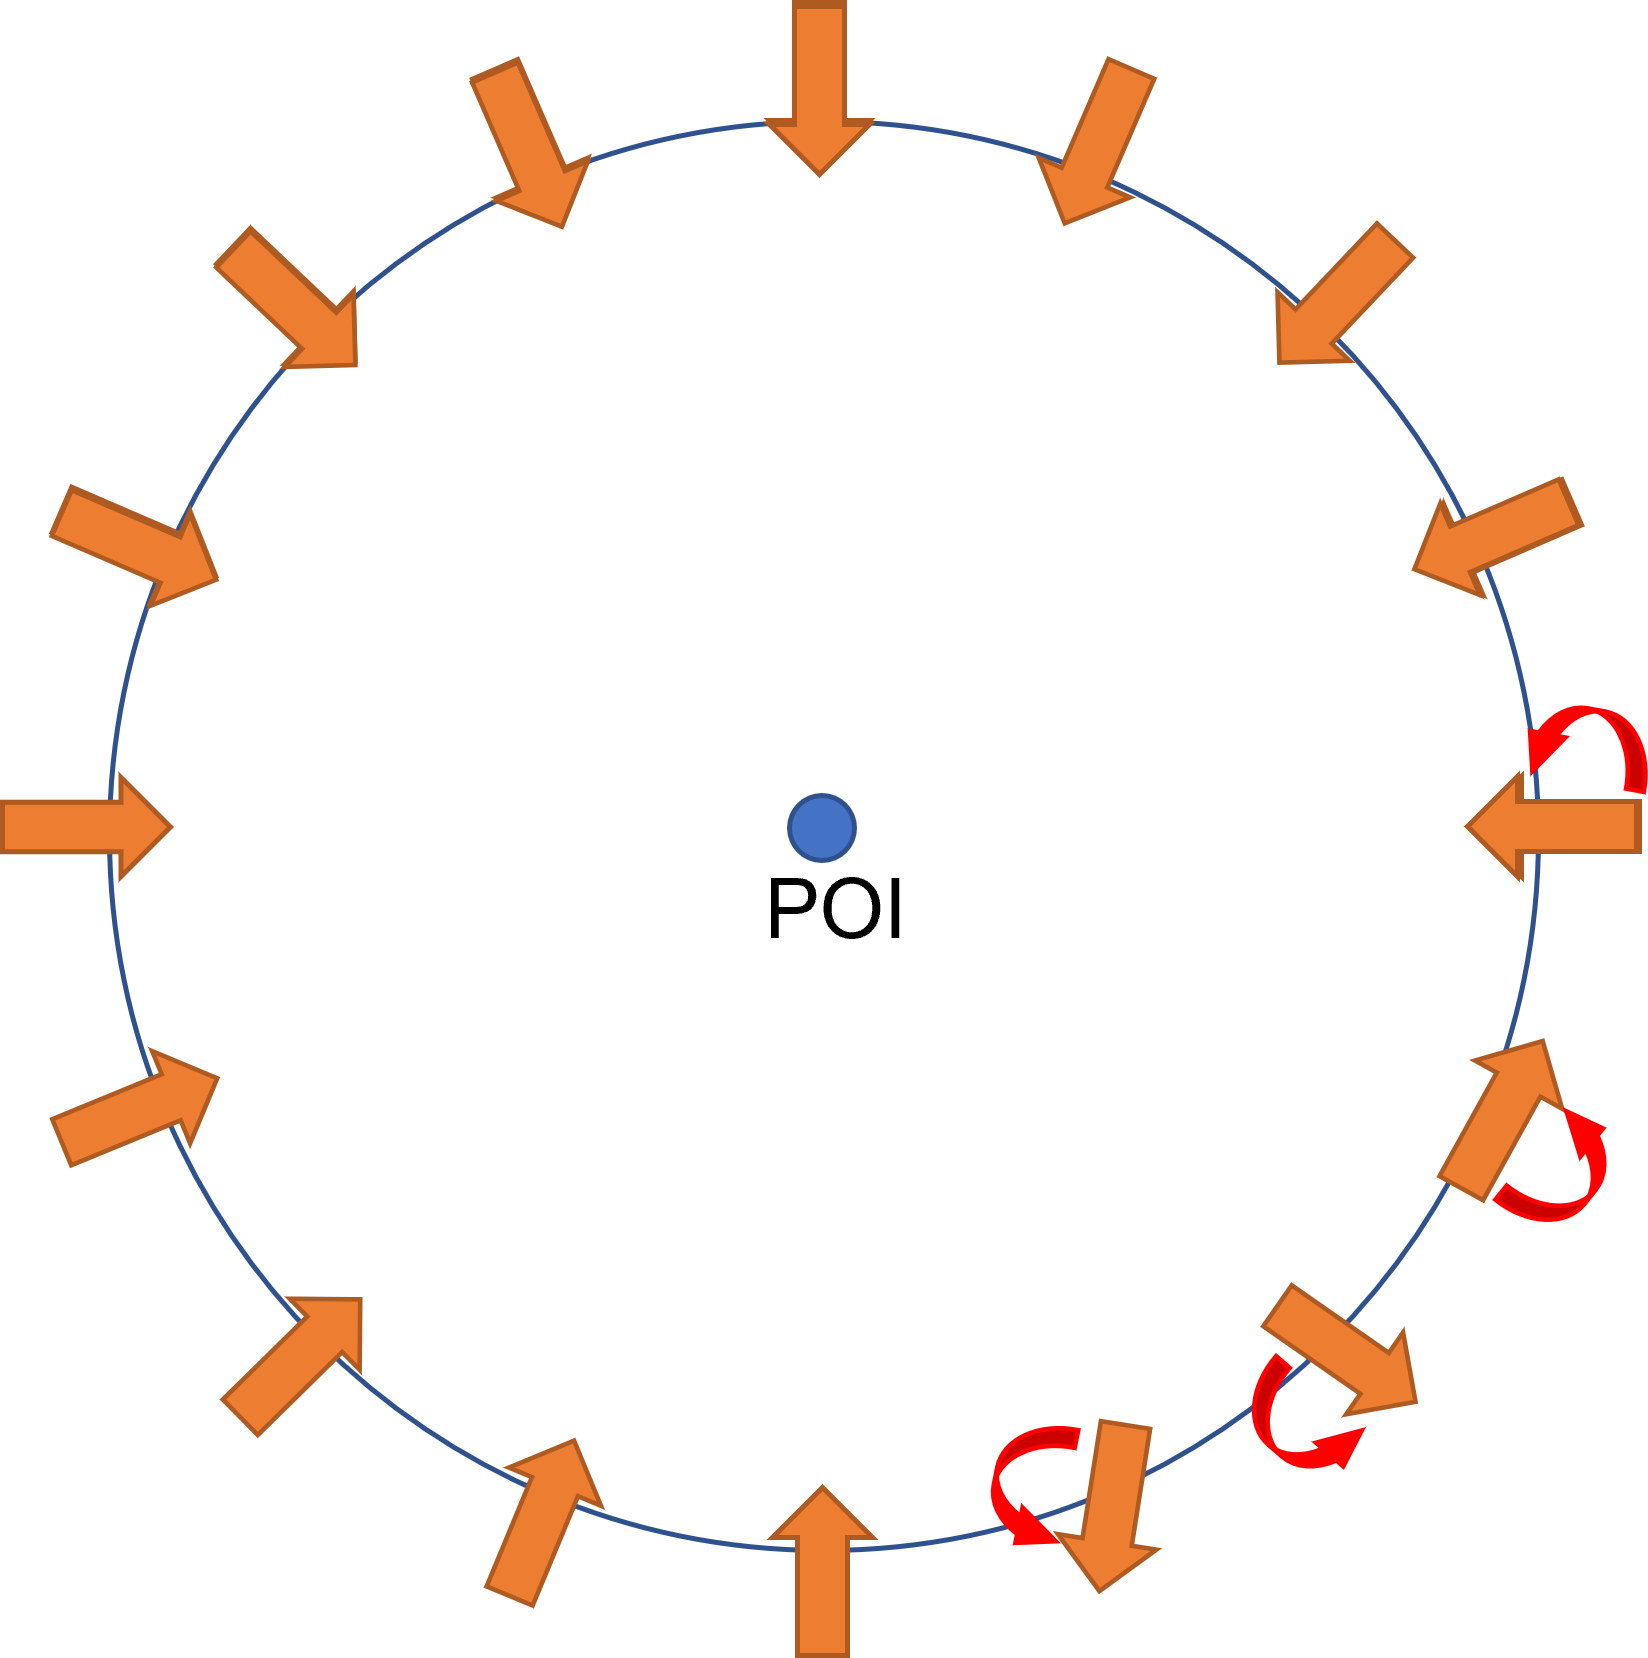
\includegraphics[width=0.5\textwidth]{images/3_wrong_transitions}
    \caption{Wrong transition on the disk}\label{fig:wrong-transition}
\end{figure}

To solve this problem, we tried different solutions: as first, we sample the next pose near to the previous one, but this solution sometime still fails.
The final solution was to sample the new position as previously defined with samplers, but instead of letting the framework to compute the intermediate poses, we manually interpolate them, and by setting frame number to one, we obtain a sequence of correctly rotating images.

\subsection{Dataset statistics}\label{subsec:dataset-statistics}
In total, we have generated 14 sequences, which are divided as follow:
\begin{table}[H]
    \center
    \begin{tabular}{|c|c|c|}
        \hline
        \textbf{Sets}           & \textbf{N. of Sequence} & \textbf{N. Image} \\ \hline
        \textbf{Training set}   & 12                      & 29.100            \\ \hline
        \textbf{Validation set} & 1                       & 1.002             \\ \hline
        \textbf{Test set}       & 1                       & 1.003             \\ \hline
        \textit{\textbf{Total}} & 14                      & 31.105            \\ \hline
    \end{tabular}\caption{Synthetic dataset statistics}
    \label{tab:synthetic-dataset-statistics}
\end{table}
Each image has dimension of 1024x308 pixels with 3 RGB channels.
The whole dateset has dimension \textbf{1.69 GB}.
\subsection{Usage}\label{subsec:usage}
By using the dataset at training time the loss function is highly variable reaching values of \textbf{thousands}, also because the \textbf{Kitti} dataset is much fluid as the trajectory and the camera rotation angles are very small, so, the sequences generated are not similar to the real dataset.
%
%%**************************************************************
%
%\input{./chapters/5_3_test_integrazione}
%
%%**************************************************************
%
%\input{./chapters/5_4_test_sistema}
%
%%**************************************************************
             % Product Design Freeze e SOP
    % !TEX encoding = UTF-8
% !TEX TS-program = pdflatex
% !TEX root = ../tesi.tex

%**************************************************************


\chapter{The State of the art}
\label{ch:state-of-the-art}
%**************************************************************
% references: https://ieeexplore.ieee.org/stamp/stamp.jsp?tp=&arnumber=9438708

%% !TEX encoding = UTF-8
% !TEX TS-program = pdflatex
% !TEX root = ../tesi.tex

%**************************************************************


\chapter{The State of the art}
\label{ch:state-of-the-art}
%**************************************************************
% references: https://ieeexplore.ieee.org/stamp/stamp.jsp?tp=&arnumber=9438708

%% !TEX encoding = UTF-8
% !TEX TS-program = pdflatex
% !TEX root = ../tesi.tex

%**************************************************************


\chapter{The State of the art}
\label{ch:state-of-the-art}
%**************************************************************
% references: https://ieeexplore.ieee.org/stamp/stamp.jsp?tp=&arnumber=9438708

%\input{./chapters/4_0_state_of_the_art.tex}
%\input{./chapters/4_2_ciclo_di_vita.tex}
%\input{./chapters/4_3_progettazione.tex}
%\input{./chapters/4_4_design_pattern_utilizzati.tex}
%\input{./chapters/4_5_codifica.tex}
%\input{./chapters/4_2_ciclo_di_vita.tex}
%\input{./chapters/4_3_progettazione.tex}
%\input{./chapters/4_4_design_pattern_utilizzati.tex}
%\input{./chapters/4_5_codifica.tex}
%\input{./chapters/4_2_ciclo_di_vita.tex}
%\input{./chapters/4_3_progettazione.tex}
%\input{./chapters/4_4_design_pattern_utilizzati.tex}
%\input{./chapters/4_5_codifica.tex}
    % !TEX encoding = UTF-8
% !TEX TS-program = pdflatex
% !TEX root = ../tesi.tex

%**************************************************************


\chapter{Experiments}
\label{ch:experiments}
%**************************************************************

%% !TEX encoding = UTF-8
% !TEX TS-program = pdflatex
% !TEX root = ../tesi.tex

%**************************************************************


\chapter{The State of the art}
\label{ch:state-of-the-art}
%**************************************************************
% references: https://ieeexplore.ieee.org/stamp/stamp.jsp?tp=&arnumber=9438708

%% !TEX encoding = UTF-8
% !TEX TS-program = pdflatex
% !TEX root = ../tesi.tex

%**************************************************************


\chapter{The State of the art}
\label{ch:state-of-the-art}
%**************************************************************
% references: https://ieeexplore.ieee.org/stamp/stamp.jsp?tp=&arnumber=9438708

%\input{./chapters/4_0_state_of_the_art.tex}
%\input{./chapters/4_2_ciclo_di_vita.tex}
%\input{./chapters/4_3_progettazione.tex}
%\input{./chapters/4_4_design_pattern_utilizzati.tex}
%\input{./chapters/4_5_codifica.tex}
%\input{./chapters/4_2_ciclo_di_vita.tex}
%\input{./chapters/4_3_progettazione.tex}
%\input{./chapters/4_4_design_pattern_utilizzati.tex}
%\input{./chapters/4_5_codifica.tex}
%\input{./chapters/4_2_ciclo_di_vita.tex}
%\input{./chapters/4_3_progettazione.tex}
%\input{./chapters/4_4_design_pattern_utilizzati.tex}
%\input{./chapters/4_5_codifica.tex}
    % !TEX encoding = UTF-8
% !TEX TS-program = pdflatex
% !TEX root = ../tesi.tex

%**************************************************************


\chapter{Implementations}\label{ch:implementations}
\intro{In this chapter we will discuss about different implementations of the models.}

%**************************************************************

\section{Dataset generation}\label{sec:dataset-generation}

%**************************************************************
\section{Models}\label{sec:models}

%**************************************************************

\section{Pose Auto-encoder}\label{sec:pose-auto-encoder}


%**************************************************************

\section{Training cycle}\label{sec:training-cycle}

%**************************************************************

    % !TEX encoding = UTF-8
% !TEX TS-program = pdflatex
% !TEX root = ../tesi.tex

%**************************************************************


\chapter{Final discussions}
\label{ch:final-discussions}
%**************************************************************
\intro{In this chapter will be discussed the results achieved.}

\section{Result Achieved}\label{sec:result-achieved}
\section{Knowledge Acquired}\label{sec:knowledge-acquired}
\section{Future Developments}\label{sec:future-developments}
\section{Personal Evaluation}\label{sec:personal-evaluation}






             % Conclusioni
%**************************************************************
% Materiale finale
%**************************************************************
    \backmatter
    \printglossaries
    % !TEX encoding = UTF-8
% !TEX TS-program = pdflatex
% !TEX root = ../tesi.tex

%**************************************************************
% Bibliografia
%**************************************************************

\cleardoublepage
\chapter{Bibliopraphy}\label{ch:bibliografia}

\nocite{*}
% Stampa i riferimenti bibliografici
\printbibliography[heading=subbibliography,title={Riferimenti bibliografici},type=book]

% Stampa i siti web consultati
\printbibliography[heading=subbibliography,title={Siti web consultati},type=online]
\printbibliography[heading=subbibliography,title={Articoli consultati},type=article]


\end{document}
